\documentclass{beamer}

\setbeamertemplate{caption}[numbered]

\usetheme{Madrid}

\usepackage{graphics}
\usepackage{amsmath}
\usepackage{xcolor}
\usepackage{physics}

\title[Wobbling Motion in Odd-Mass Nuclei] % (optional, only for long titles)
{Wobbling Motion in odd-mass nuclei}
\author[R. Poenaru] % (optional, for multiple authors)
{Robert Poenaru\inst{1,2}}
\institute[DFT @ IFIN-HH] % (optional)
{
  \inst{1}%
  Department of Theoretical Physics\newline
  IFIN-HH
  \and
  \inst{2}%
  Faculty of Physics\newline
  University of Bucharest
}
\date[\today] % (optional)
{Bucharest University Faculty of Physics 2021 Meeting}
\subject{Nuclear Physics}

\begin{document}
\maketitle
\begin{frame}
\frametitle{Table of Contents}
\tableofcontents
\end{frame}

\section{Triaxial nuclei}

\begin{frame}{Triaxiality}
\begin{itemize}
    \item Nuclear shapes: most of the nuclei are spherical or axially symmetric in the ground state.
\end{itemize}
  \begin{figure}
    \centering
    % \includegraphics[scale=0.65]{figs/prolate.pdf}
    \caption{\textbf{Spherical:} $\beta_2=0$ ; \textbf{Prolate:} $\beta_2>0$ ; \textbf{Oblate:} $\beta_2<0$}
  \end{figure}
\end{frame}

\begin{frame}{Nuclear deformation}
    \begin{block}{Nuclear surface - axially-symmetric shape}
    \begin{itemize}
    \item The shape of the nucleus can be described via the \textit{deformation parameters} $\beta,\gamma$. 
    \item They arise from the shape parametrization of the nuclear surface.
    \begin{align}
        R(\theta,\phi)=R_0\left(1+\sum_{\lambda=2}^{\infty}\sum_{\mu=0}^{\lambda}\alpha_{\lambda\mu}Y_{\lambda\mu}(\theta,\phi)\right)
    \end{align}
    \item For axial-quadrupole deformed nuclei $\beta_2=\alpha_{20}$.
    \end{itemize}
    \end{block}
\end{frame}

\begin{frame}{Deformation parameters}
    There are also deviations from \emph{axial symmetric shapes} $\to$ \textbf{triaxial shapes} (e.g. no symmetry axis).
    \begin{block}{Nuclear surface - axially-asymmetric shape}
    \begin{itemize}
    \item For nuclei with the three principal axes of different lengths (\emph{axial asymmetry}), the $\gamma$ deformation parameter emerges.
    \item Relationship between $\beta,\gamma$ and the expansion coefficients from the expression of $R(\theta,\phi)$ is given by:
    \begin{align}
        \alpha_{20}&=\beta_2\cos\gamma\\
        \alpha_{22}&=\frac{1}{\sqrt{2}}\beta_2\sin\gamma
    \end{align}
    \item $\gamma$ is a measure of asymmetry between the three \textit{moments of inertia} of the nucleus.
    \end{itemize}
    \end{block}
\end{frame}

\begin{frame}
\frametitle{Shape parameters}
\begin{figure}
    \centering
    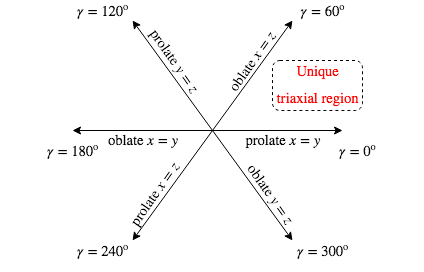
\includegraphics[scale=0.5]{figs/NuclearShapes1.png}
    \caption{The $(\beta,\gamma$) plane divided into six equivalent parts.}
    \label{fig:betagamma}
\end{figure}
\end{frame}

\begin{frame}{Wobbling motion  - clear signature for triaxiality}
\begin{columns}
\begin{column}{0.6\textwidth}
  \begin{itemize}
    \item A triaxial nucleus can rotate about any of the three axes.
    \item Rotation about the axis with the largest moment of inertia (MOI) is energetically the most favorable.
    \item The other two axes contribute to the total nuclear motion (due to the anisotropy between the MOIs) $\to$ {\color{red}This motion has an oscillating behavior}. 
    \item Spectrum: $E=E_\text{rot}+E_\text{wob}\left(n_w+\frac{1}{2}\right)$.
  \end{itemize}
\end{column}
\begin{column}{0.4\textwidth}
\begin{figure}
    \centering
      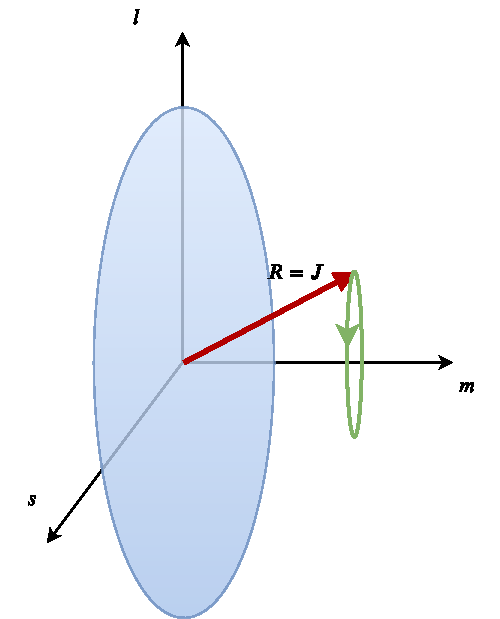
\includegraphics[scale=0.5]{figs/simpleWobbler.pdf}
      \caption{A simple wobbler.}
  \end{figure}
\end{column}
\end{columns}
\end{frame}

\begin{frame}{Wobbling motion}

\begin{columns}
    \begin{column}{0.5\textwidth}
    \begin{block}{Wobbling motion (WM)}
  \begin{itemize}
    \item Uniquely associated to triaxial structures. 
    \item It was theoretically predicted by Bohr and Mottelson more than 50 years ago (for the even-$A$ case).
    \item Experimentally confirmed for $^{163}$Lu in 2001.
  \end{itemize}
  \end{block}
  \begin{exampleblock}{Experimental evidence}
  In present, few wobblers are experimentally confirmed in the mass regions: $A\approx130,160,180$.
  \end{exampleblock}
  \end{column}
  \begin{column}{0.5\textwidth}
        \begin{figure}
          \centering
          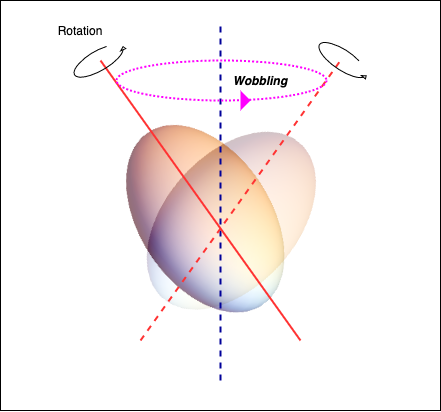
\includegraphics[scale=0.35]{figs/wobbling_drawing.png}
          \caption{Schematic representation for the nuclear wobbling motion.}
          \label{wobbling_picture}
      \end{figure}
  \end{column}
  \end{columns}
\end{frame}


\begin{frame}{Wobbling motion}
  \begin{columns}
    \begin{column}{0.47\textwidth}
    \begin{block}{Triaxial nuclei}
    The rotational angular momentum is NOT aligned along any of the body-fixed axes: it \textbf{precesses} and \textbf{wobbles} around the axes with the largest MOI. 
    \end{block}
  \begin{block}{Wobbling bands}
  Sequences of $\Delta I=2\hbar$ rotational bands that are built on different \textit{wobbling phonon excitations}.
  \end{block}
    \end{column}
    \begin{column}{0.53\textwidth}  %%<--- here
   \begin{figure}
     \centering
     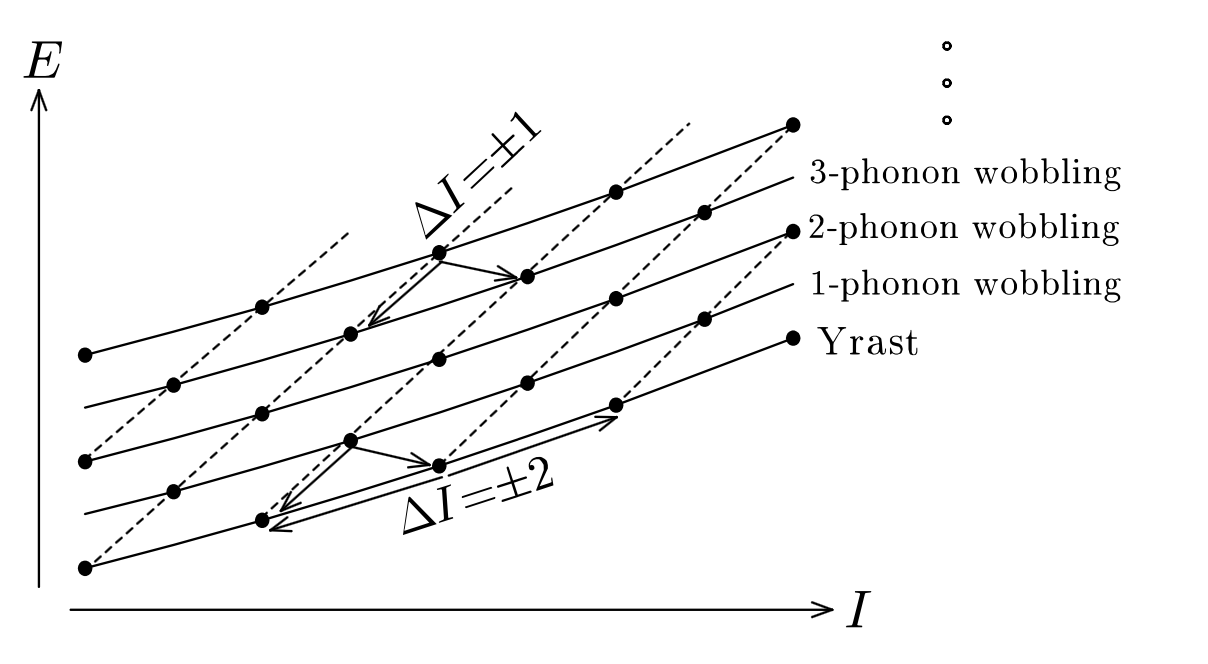
\includegraphics[scale=0.15]{figs/wobblingBands.png}
     \caption{Rotational-band structures of the wobbling motion.}
   \end{figure}
    \end{column}
    \end{columns}
\end{frame}


\begin{frame}{Particle-rotor coupling}
  \begin{block}{Wobbling motion in odd-A nuclei}  
    \begin{itemize}
      \item Coupling of a nucleon from a high j-shell with the triaxial rotor core is crucial for the wobbling phenomenon.
      \item The odd particle’s angular momentum couples to the rotor, driving the nucleus to large deformations and it also stabilizes the shape.
    \end{itemize}
  \end{block}
  \begin{exampleblock}{Odd particle}
  \begin{itemize}
      \item For nuclei with $A\approx160$, the odd $\pi i_{13/2}$ is the \emph{intruder} which drive the isotope to very high deformations (up to $n_w=3$ wobbling phonon number).
      \item For nuclei with $A\approx180$, the odd $\pi h_{9/2}$ and $\pi i_{13/2}$ are the \emph{intruders} which drive the system to very high deformations.
  \end{itemize}
  \end{exampleblock}
\end{frame}


\begin{frame}{Wobbling regimes}
  Frauendorf et al (2014) formulated two possible wobbling modes in the case of $odd-A$ nuclei.
  \begin{block}{$\ $}
    \begin{description}
      \item[Longitudinal wobbling (WL)] the quasiparticle's angular momentum $j$ is \emph{aligned} with the rotational axis of the system ($m$-axis for triaxial nuclei)
      \item[Transverse wobbling (TW)] the quasiparticle's a.m. $j$ is \emph{perpendicular} to the rotational axis ($m$); so it is parallel with either the long ($l$) axes or the short ($s$ axes). 
    \end{description}
  \end{block}
\end{frame}

\begin{frame}{LW vs TW - graphical representation}
  \begin{columns}
    \begin{column}{0.5\textwidth}  %%<--- here
      \begin{figure}
        \centering
        \includegraphics[scale=0.6]{figs/LongitudinalWobbler.pdf}
      \end{figure}
    \end{column}
    \begin{column}{0.5\textwidth}
      \begin{figure}
        \centering
  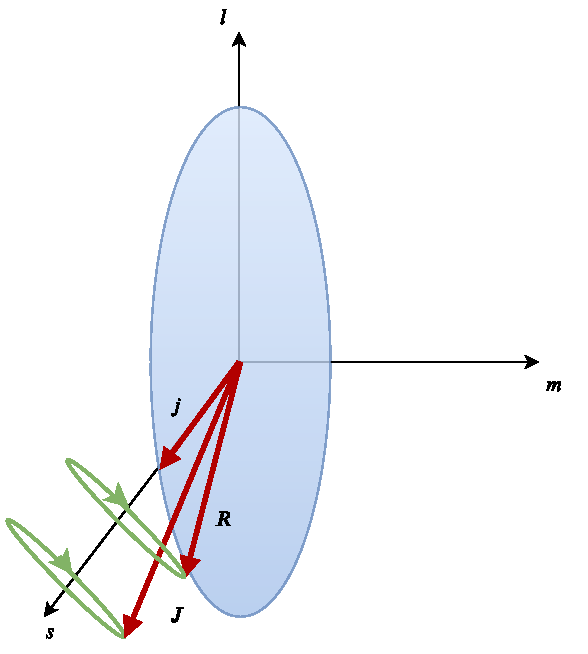
\includegraphics[scale=0.6]{figs/transverseWobbler.pdf}

      \end{figure}
    \end{column}
    \end{columns}

\end{frame}

\section{Theoretical Formalism}

\begin{frame}{Theoretical framework}
  The odd-mass system consists of an {\color{red}even-even core} (described by a triaxial rotor Hamiltonian {\color{red}$H_\text{rot}$}) and a single {\color{blue}$j$-shell nucleon} described by its single-particle Hamiltonian {\color{blue}$H_\text{sp}$}.
  \par \textbf{Total system:}
  \begin{align}
    &H={\color{red}H_\text{rot}}+{\color{blue}H_\text{sp}}=\\
&{\color{red}\sum_{k=1,2,3}A_k(I_k-j_k)^2}+{\color{blue}\epsilon_j+\frac{V}{j(j+1)}\left[\cos\gamma(3j_3^2-\mathbf{j}^2)-\sqrt{3}\sin\gamma(j_1^2-j_2^2)\right]}
  \end{align}
  \par {\footnotesize \textbf{Solving the Hamiltonian in semi-classical approach for $^{163}Lu$}: \textit{R. Poenaru and A. A. Raduta, International Journal of Modern Physics E, 2150033, 2021}.}
  \par {\footnotesize \textbf{For $^{135}Pr$}: \textit{A. A. Raduta and R. Poenaru, Journal of Physics G, 015106, 2020}.}
\end{frame}

\begin{frame}{Energy function - Semiclassical approach}
      The eigenvalues for $\hat{H}=H_{rot}+H_{sp}$ are obtained by solving the \emph{variational principle}:
  \begin{align}
    \delta \int_0^t\bra{\Psi_{IjM}}\hat{H}-i\frac{\partial}{\partial t'}\ket{\Psi_{IjM}}dt'=0. \label{varp}
  \end{align}
  The trial function $\ket{\Psi_{IjM}}$ is a direct product $\ket{\psi}_\text{core}\otimes\ket{\phi}_\text{s.p.}$.
    From Eq. \ref{varp}, one obtains the \emph{classical equations of motion} in the canonical form:
  \begin{align}
    \frac{\partial \mathcal{H}}{\partial r}=\dot{\varphi}\ ;\ \frac{\partial\mathcal{H}}{\partial\varphi}=-\dot{r}\\
    \frac{\partial \mathcal{H}}{\partial t}=\dot{\psi}\ ;\ \frac{\partial\mathcal{H}}{\partial \psi}=-\dot{t}
  \end{align}
\end{frame}


\begin{frame}{Classical energy function}
Considering the \emph{energy function} as the average of the Hamiltonian on the trial function:
  \begin{align}
    \mathcal{H}\equiv\bra{\Psi_{IjM}}H\ket{\Psi_{IjM}}
  \end{align}
  \begin{block}{Harmonic frequencies}
  \begin{itemize}
      \item The energy function is \emph{minimal} in the point $\mathcal{P}_{min}$ when $A_1<(A_2,A_3)$.
      \item Linearizing the equations of motion around the minimum point of $\mathcal{H}$, one obtains a harmonic motion for the system, with the \emph{frequencies} given by:
  \begin{align}
    \Omega^4+B\Omega^2+C=0 \label{omegaeq}
  \end{align}
  \item $B$ and $C$ functions that depend on: \textbf{the inertia factors $A_k$, single particle potential strength $V$ and the triaxiality parameter $\gamma$}.
  \end{itemize}  
  \end{block}
\end{frame}

\begin{frame}{Semiclassical wobbling energies}
\begin{block}{Harmonic Frequencies II}
\begin{itemize}
    \item The two real and positive solutions for Eq. \ref{omegaeq}: $\Omega_1$ and $\Omega_2$ are called \emph{the wobbling frequencies}.
    \item They represent the harmonic-like behavior of the wobbling motion in odd-A nuclei.
  \item In our model, the pair of frequencies $({\color{blue}\Omega_1^I},{\color{red}\Omega_{2}^I})$ is associated with the rotational motion of the {\color{blue}core} and the {\color{red}odd particle}, respectively.
\end{itemize}
\end{block}
\begin{alertblock}{Energy spectrum}
\begin{align}
    E_I&={\color{cyan}\epsilon_{j}}+{\color{magenta}\mathcal{H}_\text{min}(I)}+\left[{\color{blue}\Omega_1^I\left(n_{w_1}+\frac{1}{2}\right)}+{\color{red}\Omega_2^I\left(n_{w_2}+\frac{1}{2}\right)}\right] \label{wobbling_formula}
  \end{align} 
  Terms: {\color{cyan}{single particle energy}}, {\color{magenta}energy in the minimum point} and [harmonic-like motion].
\end{alertblock}
\end{frame}

\section{New results for Au wobblers}  

\begin{frame}
    \frametitle{{\footnotesize \emph{preliminary}} Results for $^{183}$Au}
\textit{S. Nandi et. al. (PRC, 132501, 2020)} - First Observation of Multiple Transverse Wobbling Bands in $^{183}$Au.
    \begin{columns}[c] 
    \column{.5\textwidth}
     \begin{figure}
         \centering
         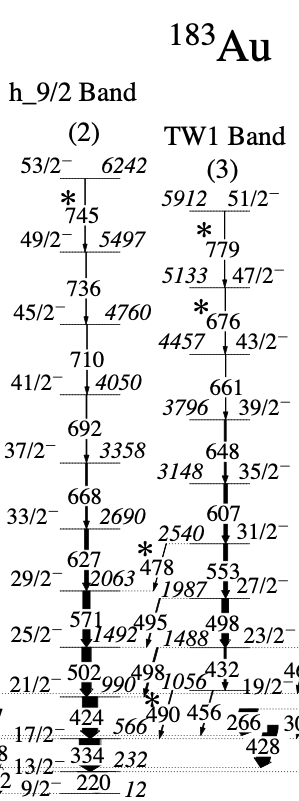
\includegraphics[scale=0.15]{figs/negative_Au183.png}
         \caption{The first wobbling sequence (negative parity states).}
         \label{au183negative}
     \end{figure}
    \column{.5\textwidth}
     \begin{figure}
         \centering
         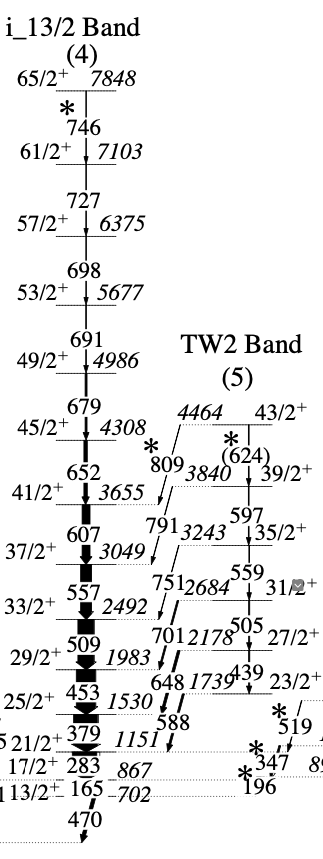
\includegraphics[scale=0.15]{figs/positive_Au183.png}
         \caption{The second wobbling sequence (positive parity states).}
         \label{au183positive}
     \end{figure}
    \end{columns}
\end{frame}

\begin{frame}{Fitting the model}
    We tested our formalism by fitting the expression of the energy formula (Eq. \ref{wobbling_formula}) to the experimental data for the wobbling spectrum of both isotopes.
    \begin{block}{Parametrization: negative parity bands}
    \begin{itemize}
    \item The odd-particle: $h_{j=9/2}$ proton.
    \item ground-state band: $(n_{w_1},n_{w_2})=(0,0)$.
    \item second wobbling band: $(n_{w_1},n_{w_2})=(1,0)$.
    \end{itemize}
    \end{block}
    \begin{block}{Parametrization: positive parity bands}
    \begin{itemize}
    \item The odd-particle: $i_{j=13/2}$ proton.
    \item ground-state band: $(n_{w_1},n_{w_2})=(0,0)$.
    \item second wobbling band: $(n_{w_1},n_{w_2})=(1,0)$.
    \end{itemize}
    \end{block}
\end{frame}

\begin{frame}
    \frametitle{{\tiny \emph{preliminary}} Results for $^{183}$Au II}
    \begin{columns}[c] 
    \column{.5\textwidth}
     \begin{figure}
         \centering
         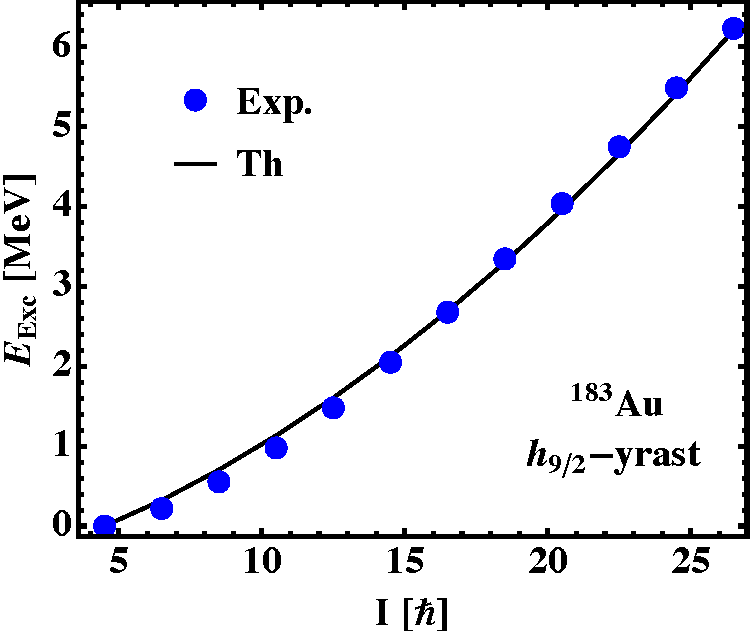
\includegraphics[scale=0.4]{figs/Au_183_plot1Negative.pdf}
         \caption{First band (negative parity).}
     \end{figure}
    \column{.5\textwidth}
     \begin{figure}
         \centering
         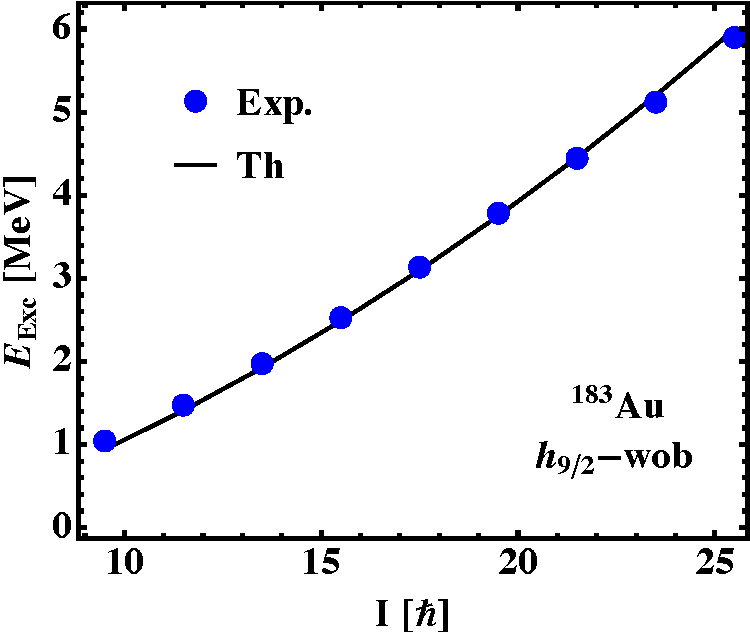
\includegraphics[scale=0.4]{figs/Au_183_plot2Negative.pdf}
         \caption{Second band (negative parity).}
     \end{figure}
    \end{columns}
    \par $rms\approx79$ keV.
    \par $\mathcal{I}_1$=86.71, $\mathcal{I}_2$=10.30, $\mathcal{I}_3$=4.36 $\hbar^2/\text{MeV}^{-1}$
    \par $V=0.1747387$ MeV, $\gamma=21.23^o$ ($\gamma_\text{exp}\approx 20$).
\end{frame}

\begin{frame}
    \frametitle{{\tiny \emph{preliminary}} Results for $^{183}$Au III}
    \begin{columns}[c] 
    \column{.5\textwidth}
     \begin{figure}
         \centering
         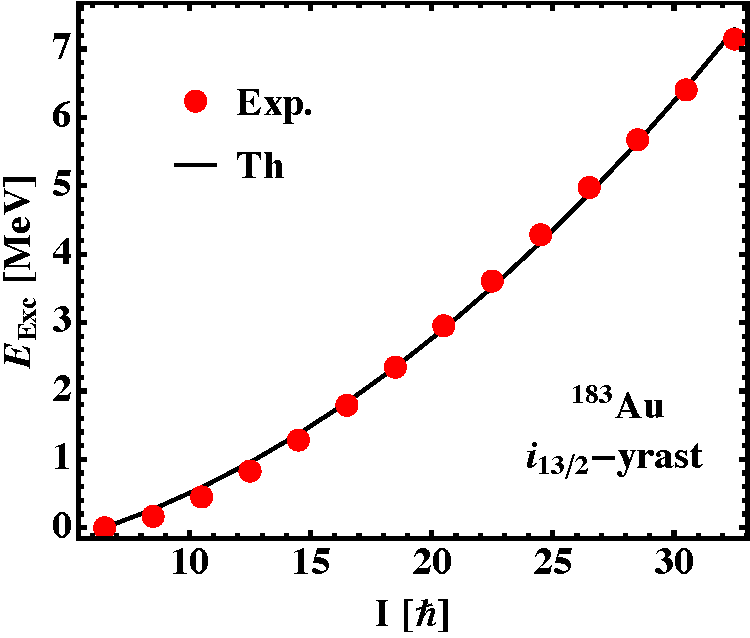
\includegraphics[scale=0.4]{figs/Au_183_plot1Positive.pdf}
         \caption{First band (positive parity).}
     \end{figure}
    \column{.5\textwidth}
     \begin{figure}
         \centering
         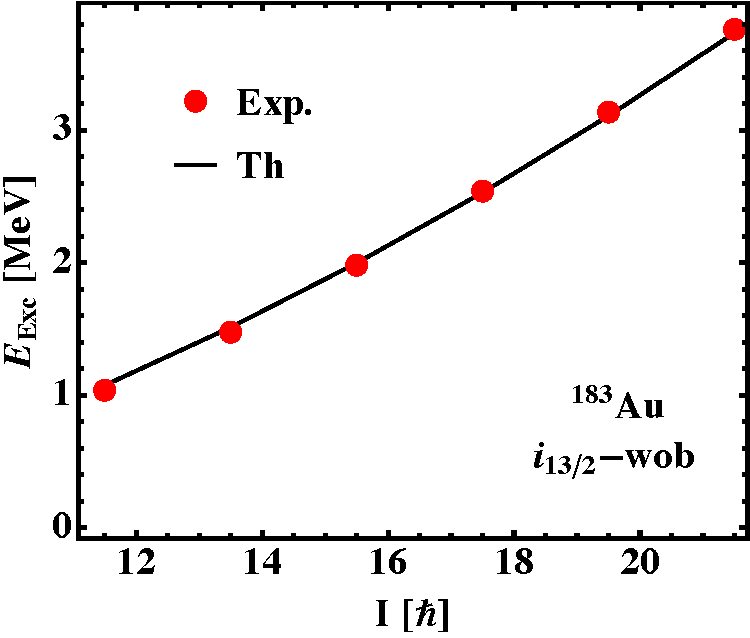
\includegraphics[scale=0.4]{figs/Au_183_plot2Positive.pdf}
         \caption{Second band (positive parity).}
     \end{figure}
    \end{columns}
    \par $rms\approx73$ keV.
    \par $\mathcal{I}_1$=83.4, $\mathcal{I}_2$=3.63, $\mathcal{I}_3$=26 $\hbar^2/\text{MeV}^{-1}$
    \par $V=1.95$ MeV, $\gamma=19.7^o$ ($\gamma_\text{exp}\approx 21$).
\end{frame}

\begin{frame}
    \frametitle{{\tiny \emph{preliminary}} Results for $^{187}$Au}
    \begin{columns}[c] 
    \column{.65\textwidth}
    \begin{block}{Parametrization}
    \begin{itemize}
        \item \textit{N. Senhsarma et. al. (PRL, 052501, 2020) showed evidence for Longitudinal Wobbling in ${187}$Au.}
        \item Two such wobbling bands have been confirmed (Longitudinal character).
        \item The odd proton $h_{11/2}$ is coupling to the triaxial core.
        \item ground-state band: $(n_{w_1},n_{w_2})=(0,0)$.
        \item second wobbling band: $(n_{w_1},n_{w_2})=(1,0)$.
    \end{itemize}
    \end{block}
    \column{.35\textwidth}
     \begin{figure}
         \centering
         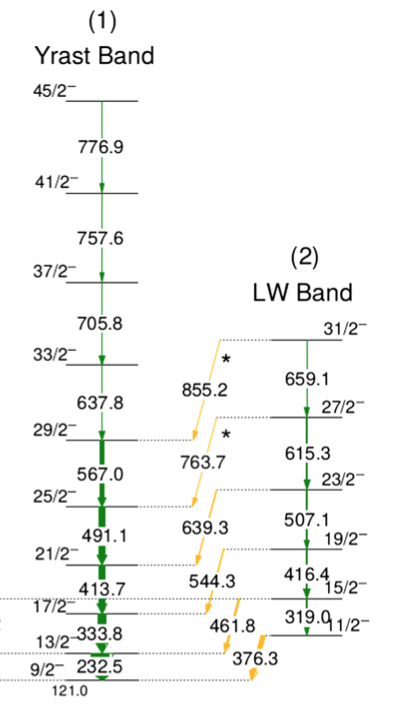
\includegraphics[scale=0.2]{figs/spectrum_Au187.png}
         \caption{Experimental evidence of wobbling excitations in $^{187}$Au.}
     \end{figure}
    \end{columns}
\end{frame}

\begin{frame}
    \frametitle{{\tiny \emph{preliminary}} Results for $^{187}$Au II}
    \begin{columns}[c] 
    \column{.5\textwidth}
     \begin{figure}
         \centering
         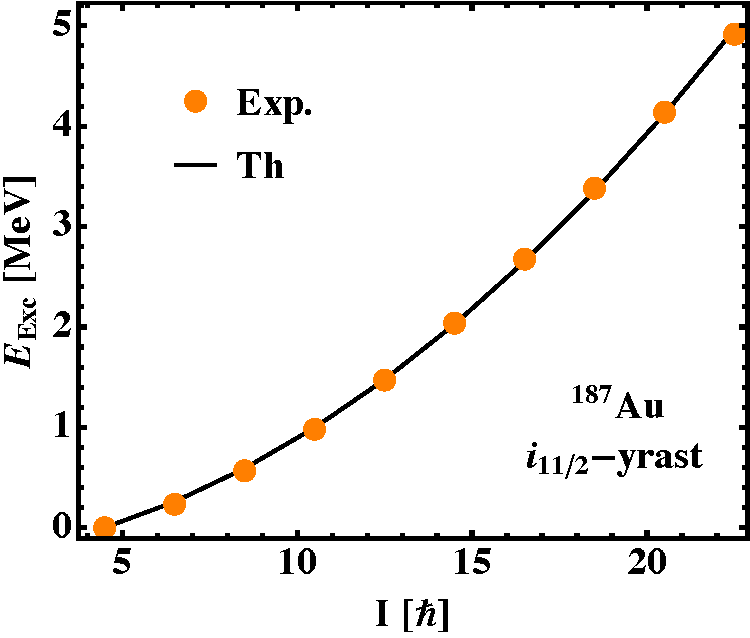
\includegraphics[scale=0.4]{figs/Au_187_1.pdf}
         \caption{First band (positive parity).}
     \end{figure}
    \column{.5\textwidth}
     \begin{figure}
         \centering
         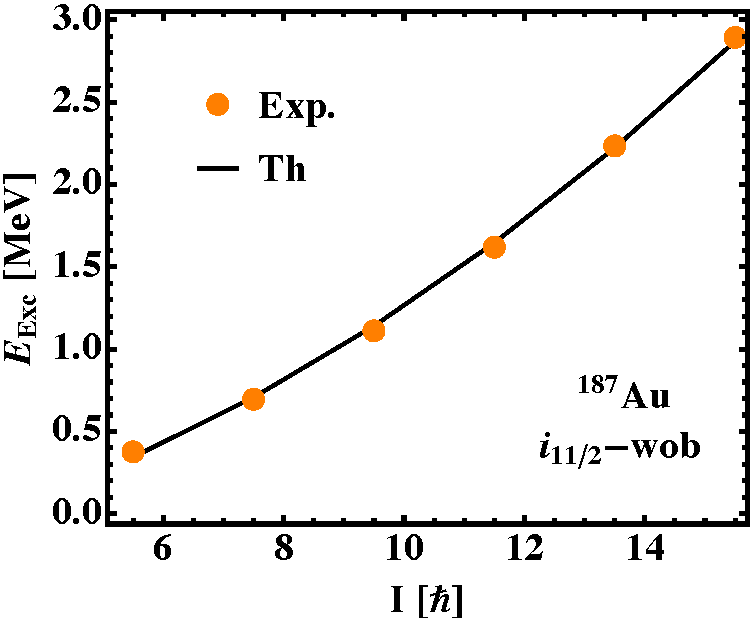
\includegraphics[scale=0.4]{figs/Au_187_2.pdf}
         \caption{Second band (positive parity).}
     \end{figure}
    \end{columns}
    \par $rms\approx23$ keV.
    \par $\mathcal{I}_1$=55.1, $\mathcal{I}_2$=3.81, $\mathcal{I}_3$=19.56 $\hbar^2/\text{MeV}^{-1}$
    \par $V=2.02$ MeV, $\gamma=20^o$
\end{frame}

\section{Conclusions}

  \begin{frame}
  \centering
    \Large{Thank you for your attention!}
  \end{frame}

\end{document}